\section{Benchmark Description}

%\subsection{Overview}
According to our research and survey,
%we found that a suite of easy-to-use NFV benchmark is indeed.
the most urgent demand of an NFV benchmark is 
to reduce the deployment time which includes 
setting up virtualization platform and its network environment, 
packing and managing VNF images, 
writing scripts to automatically start NFs and chain them up. 
Another requirement of the benchmark is to provide 
representative VNF with widely accepted chaining policies, 
as well as proper workload generator to drive the chains.
A suite of off-the-shelf benchmark can also 
reduce the time spent on NF selecting. 

In this section, we first describe the overall architect of our benchmark 
and the simple steps for a user to do deployment and testing. 
Then we introduce the NFs and chains we use. 
And give out possible use cases of our benchmark.

%So, a selected suite of representative VNF
%with widely accepted chaining policy
%and proper workload generator is needed.
%%The idea of our work is based on an observation that
%Second, a well-designed benchmark with a bunch of
%pre-written scripts to automate the deployment process can effectively save time.
%Since NFV involves multi-layers in the whole software stack,
%the automation process includes VNF image packaging,
%NF allocation, networking config, forwarding rules installation,
%connection testing, and metrics measurement.
%%The goal and challenges of the work
%
%The goal of our work is to provide a benchmark suite
%with the following three characteristics:
%1) Representing typical NFs 2) Easy to use 3) Plenty metrics for measurement.

%Challenges:
%
%Representative NF
%
%K8s+ovs
%
%measurement

\subsection{Benchmark}

\begin{figure}[!t]
\centering
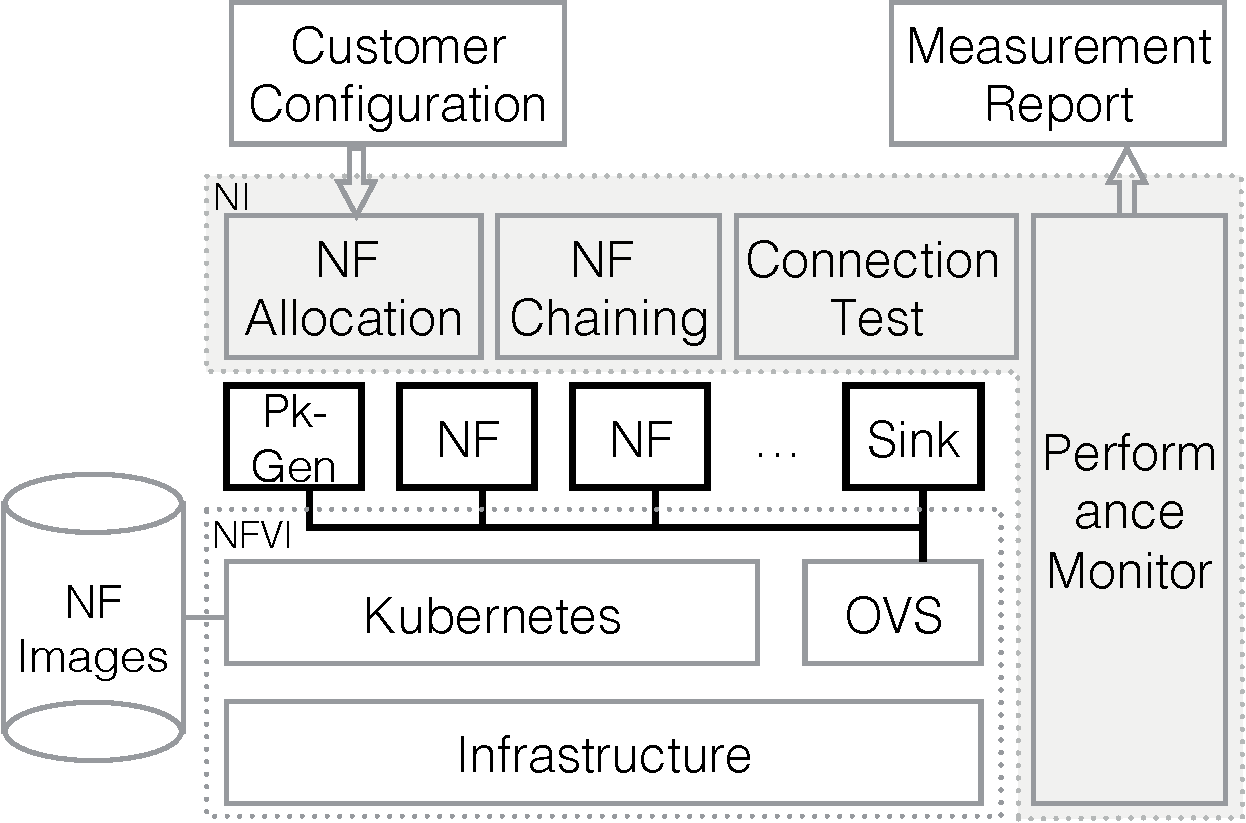
\includegraphics[width=3.3in]{fig/design2.pdf}
\caption{An overview of our benchmark design.}
\label{design}
\end{figure}

%Framework

The overall architecture of our benchmark is shown in Figure \ref{design}.
It has three main parts, NFVI, NF services and NI.
NFVI (NFV Infrastructure) consists of hardware resources
including compute, storage and network. 
NF services are deployed upon NFVI, forming a service chain. 
To leverage docker's light-weight isolation 
and its convenience of packing a runtime environment, 
we chose to use Kubernetes as the infrastructure management framework, 
which manages the physical cluster as well as the dockers and images. 
OVS is used as the data path, 
and forwarding rules installed on OVS chains up the NF services.
The details of our network settings will be introduced in section 4.1.

NI (NfvInsight) is the key component of our benchmark, 
which consists of a bunch of scripts 
to automate the process of NF chain deployment.
To simplify its usage, 
users are supposed to run only one command to start the test,
and touch only two files, 
one configuration file and one measurement report.
NI reads in the customer configuration file, 
parse it, and generate scripts to start docker, config network, and run NF.
%It does NF allocation and chaining automatically leveraging NFVI management framework.
Furthermore, it does connection test and performance monitoring during test running.

The process for a researcher to use the benchmark includes five simple steps:

\begin{itemize}
\item[\textbf{1.}]{}\textbf{Run the pre-install script.}
In the first step, users need to install Kubernetes, OVS
and Openflow controller for their physical server cluster.
%Kubernetes is an open-source system for automating deployment, scaling,
%and management of containerized applications.
To force forwarding packets cross nodes,
OVS bridge and Openflow global control is needed.

\item[\textbf{2.}]{}\textbf{Run the image building script.}
We provide DOCKERFILE to build images for each VNF listed in Table \ref{nfs},
A private registry is needed to manage the images,
so that Kubernetes can create containers distributely using local images.

\item[\textbf{3.}]{}\textbf{Write config file.}
This config file is the only file needs user edit.
It includes choice of testing chain,
mapping between physical server and docker,
resource configuration of each docker,
host network and other NF specific configurations.
To config each NF working in the demanded mode,
we provide pre-written config files for each NF.

\item[\textbf{4.}]{}\textbf{Run test with one click.}
Users can run the test by executing only one command.
NI does a series automate processes.
First it reads the configuration file edited by users and rewrites the related scripts,
which including container deployment scripts and NF config files.
Then the NF Allocation module deploys containers according to user configuration.
When containers are started and their status turn to `ready',
NF Chaining module adds virtual NIC for each container,
connects them to OVS bridge,
and installs Openflow forwarding rules according to the chaining policy.
To check whether the chain works,
the Connection Test module send a TCP request
from the packet generator and check if it gets response from Apache server.
If the connection test is passed,
the test is run and metric measurement begins.

\item[\textbf{5.}]{}\textbf{Get the report.}
The Performance Monitor module does metric measurement
and output a report.

\end{itemize}


\subsection{VNF}

\begin{table}[!b]
\newcommand{\tabincell}[2]{\begin{tabular}{@{}#1@{}}#2\end{tabular}}
\centering
\begin{tabular}{|c|c|c|}\hline
\textbf{Category} & \textbf{NF} & \tabincell{c}{\textbf{Workload}\\\textbf{Generator}}\\\hline
IMS & Clearwater & SipP \\\hline
IDS & Snort & \multirow{4}{*}{Httperf} \\\cline{1-2}
NAT & iptables & \\\cline{1-2}
L4 Load Balancer & Haproxy & \\\cline{1-2}
L7 Cache & Squid & \\\hline
\end{tabular}
\caption{NFs included in our benchmark.}
\label{nfs}
\end{table}

To select representative VNF,
%Since VNFaaS (VNF as a Service) and IMS are
%the most prevalent NFV use cases,
%we choose to .
We reviewed papers on NFV and find out
all the open source implementations has been used.
We categorized them into several kinds according to their function,
and selected the VNF which needs no modification of the kernel.
NI provides DOCKERFILE to packet VNF into docker images,
and provides pre-wirtten config files to
config each VNF working in the way as demanded.
Table \ref{nfs} lists information of the VNF
and the workload generator used.
Because iptables, Haproxy and Squid need real tcp requests,
packet trace replay cannot make them work properly,
we use Httperf to generate requests
and Apache Server to respond the requests.
The following are the brief introduction of the VNF:

\begin{itemize}
\item{}
Clearwater \cite{noauthor_project_nodate} is an open source implementation of IMS (the IP Multimedia Subsystem) designed from the ground up for massively scalable deployment in the Cloud to provide voice, video and messaging services to millions of users.

\item{}
Snort \cite{} is an open source intrusion prevention system
capable of real-time traffic analysis and packet logging.
We config it working under intrusion detection model.

\item{}
Iptables \cite{}
We set particular rule to use iptables as DNAT and SNAT.

\item{}
Haproxy \cite{} is a reliable, high performance TCP or HTTP load balancer.
We config it working under TCP mode to do L4 load balancing.

\item{}
Squid \cite{} is a caching proxy for the Web supporting HTTP, HTTPS, FTP, and more. It reduces bandwidth and improves response times by caching and reusing frequently-requested web pages.
\end{itemize}

\subsection{VNF Chain}

\begin{table*}[!t]
\newcommand{\tabincell}[2]{\begin{tabular}{@{}#1@{}}#2\end{tabular}}
\centering
\begin{tabular}{|l|l|l|}\hline
\textbf{} & \multicolumn{1}{c|}{\textbf{Sample Service Function Chains}} & \multicolumn{1}{c|}{\textbf{Chains in NI}} \\\hline
SFC1 & EdgeFW & Httperf $\to$ iptables $\to$ Apache \\\hline
SFC2 & EdgeFW $\to$ ADC & Httperf $\to$ iptables $\to$ Haproxy $\to$ Apache \\\hline
SFC3 & EdgeFW $\to$ ADC $\to$ AppFW & Httperf $\to$ iptables $\to$ Haproxy $\to$ Snort $\to$ Apache \\\hline
SFC4 & WOC $\to$ EdgeFW $\to$ ADC $\to$ AppFW & Httperf $\to$  Squid $\to$ iptables $\to$ Haproxy $\to$ Snort $\to$ Apache \\\hline
\end{tabular}
\caption{Sample VNF service function chains and chains provided by our benchmark.}
\label{chains}
\end{table*}

To find representative NF chaining policies,
we referred to IETF Service Function Chaining Use Cases
In Data Centers \cite{draft-ietf-sfc-dc-use-cases-06}.
The standard provides several sample service chains,
as listed in Table \ref{chains}, the second column.
The sample chains are connected by four network function concepts.
Definitions of each function concepts are given in the standard file,
and are listed in the following part of the paper.
The definitions are generalized,
actual implementations may vary and have functions overlapped.
We form the chains in our benchmark using the open sources
implementations in Table \ref{nfs} according to the sample chains.
The chains in NI are listed in Table \ref{chains}, the right column.

\begin{itemize}
\item
Edge Firewall (EdgeFW): Service functions such as VPN, DHCP, NAT, IP-Audit, Protocol Inspection, DPI etc., with policies primarily focusing on threats external to the data center.

\item
Application Delivery Controller (ADC): Service Function that distributes traffic across a pool of servers (applications) for efficient resource utilization, application scaling as well as to provide high availability among others.

\item
Application Firewall (AppFW): Service Function that isolates traffic within a segment or protects from application specific threats. This falls into the same class as DPI but deployed much closer to the applications. It is an intra-segment firewall.

\item
Web Optimization Control (WOC): Service functions to optimize the use of WAN link bandwidth, improve effective user throughput and latencies leading to overall improved user experience. WOC includes various optimizers such as compression, de-duplication, congestion control, application specific optimizers, etc. %WOC requires peers at either end of the WAN link to perform optimizations. The scope of this document is limited to the DC side of the WAN link.
\end{itemize}

% \begin{figure}[t]
% \label{cdf}
% \centering
% 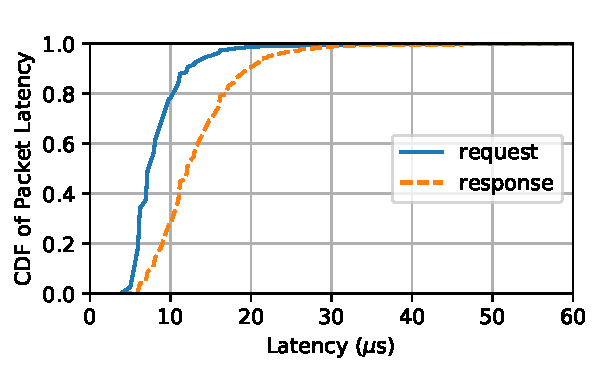
\includegraphics[width=3.3in]{cdf_chain1.pdf}
% \caption{Per-packet latency}
% \end{figure}

% \begin{figure}[t]
% \label{cdf}
% \centering
% 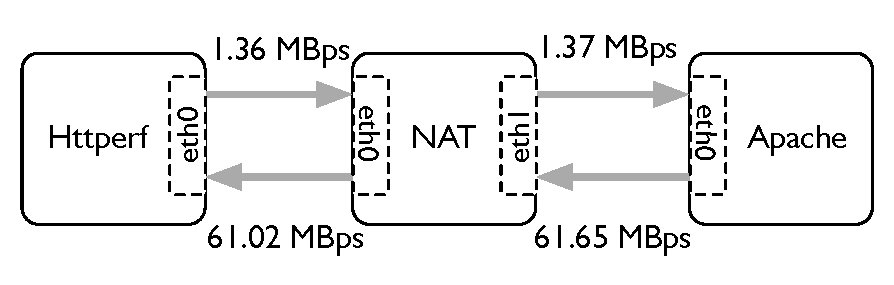
\includegraphics[width=3.3in]{throughput_chain1.eps}
% \caption{Throughput}
% \end{figure}

% \begin{figure}[t]
% \label{cdf}
% \centering
% 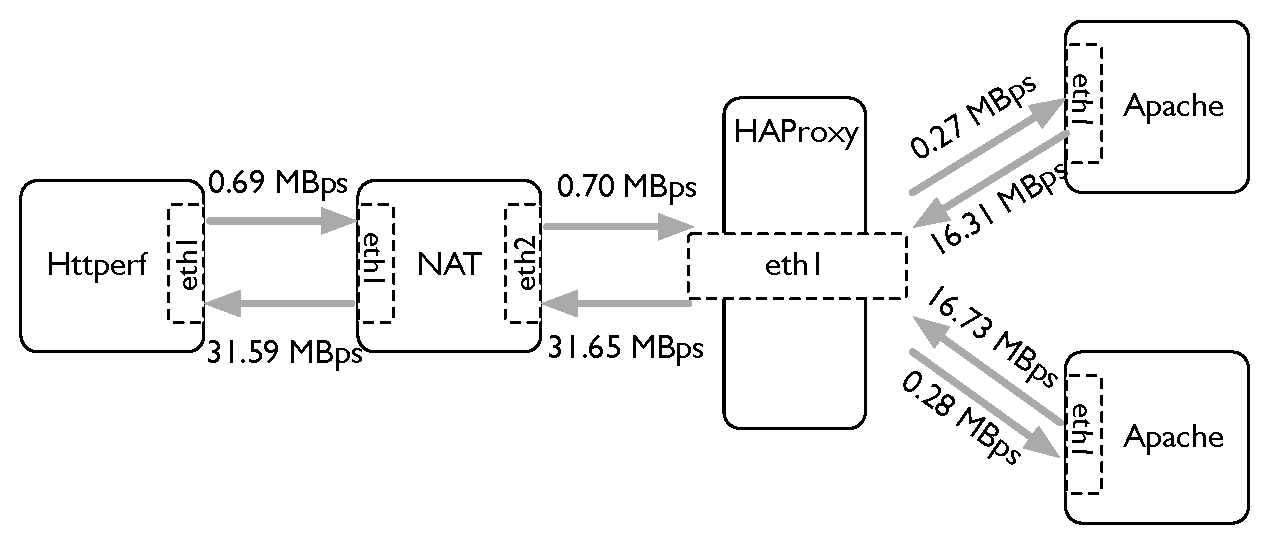
\includegraphics[width=3.3in]{throughput_chain2.eps}
% \caption{Throughput}
% \end{figure}


\subsection{Use Case for NfvInsight}
First, for all these researches, a universally used baseline is lacked
for comparison experiments.

\section{Implementation}
\subsection{Multiple Server}
\subsection{Image Registry}
\subsection{Config File}
\subsection{Auto Deploy}
\subsection{Measurement}

